% !TeX program = xelatex
% !TEX encoding = UTF-8 Unicode

\documentclass[9pt]{article}
\usepackage{hyperref}
\usepackage{ulem} 
\usepackage{mathtools}
\usepackage{enumitem}
\usepackage{color,soul}
\usepackage{inputenc}
\usepackage[margin=2.75cm]{geometry}
\usepackage{xcolor}
\usepackage{listings}

% TODO Modificare questi parametri per scrivere un bash più bello

\lstset{basicstyle=\ttfamily,
	showstringspaces=false,
	commentstyle=\color{blue},
	keywordstyle=\color{red}
}
\lstset{
	language=bash,
	basicstyle=\ttfamily
}

\begin{document}

\title{Shell Scripting 2020: Week }
\author{\textbf{Stefan Ciprian Voinea}\\Student number: 015383372}
\maketitle

%\begin{figure}[h!]
%	\centering
%	\includegraphics[width=12cm]{autoconfiguration.png}
%	\caption{IPv6 Autoconfiguration example}
%	\label{fig:autoconfig}
%\end{figure}

\begin{enumerate}
	
	\setcounter{enumi}{30}
	
	\item \textbf{ASCII art}
	
		Output of the execution:
		\begin{figure}[h!]
			\centering
			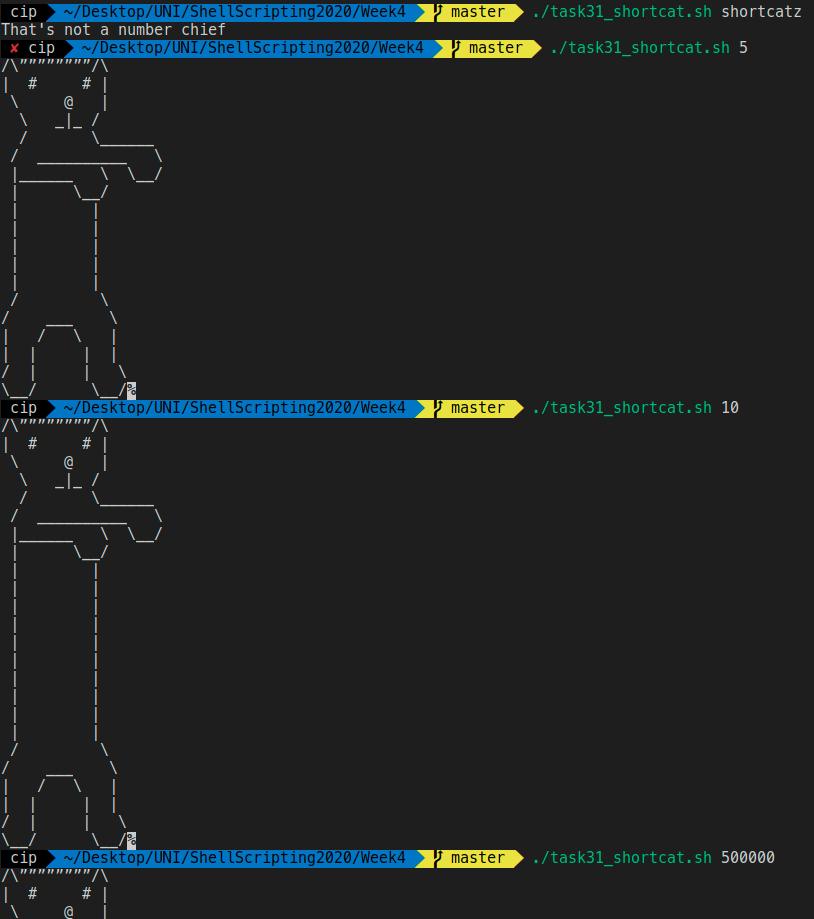
\includegraphics[width=14cm]{img/31.png}
		\end{figure}
	
		\newpage
		Contents of the \texttt{task31\_shortcat.sh} file:
		\begin{lstlisting}
belly_lines=$1

re='^[0-9]+$'
if ! [[ $belly_lines =~ $re ]] 
then
    echo "That's not a number chief"
    exit 1
fi

if [ $belly_lines -gt 1 ]
then
    head -n 8 shortcat.txt
    for i in $(seq 1 $belly_lines)
    do 
        sed "9q;d" shortcat.txt
    done
    tail -n 6 shortcat.txt
else
    echo "Nope"
fi
		\end{lstlisting}


	\item \hl{\textbf{Plotting}}
	\item \hl{\textbf{Let's plot some real data points}}
	\item \hl{\textbf{Let's put some context}}
	\item \hl{\textbf{Let's generalize}}
	\item \hl{\textbf{Let's make more refined commands}}
	
\end{enumerate}

\end{document}